\documentclass[12pt, a4paper, titlepage]{article}

\usepackage[spanish]{babel}
\usepackage[utf8]{inputenc}
\usepackage{graphicx}

% Margin set to a4wide
\usepackage{geometry}
\usepackage{layout}

\geometry{
  left=2cm,
  right=2cm,
  top=3.5cm,
  bottom=3cm
}

\usepackage{listings}
\usepackage{dirtree}
\usepackage{chicago}
\usepackage{multicol}
\usepackage{hyperref}

\def\labelitemi{$\bullet$}

\linespread{1.3}

\title{
  \large{Diseño e Implementación de Compiladores}\\
  \huge{Diseño de un compilador para \textsc{compi}}
}

\author{
  Cardellino, Cristian $\cdot$ Leberle, Maico $\cdot$ Soldevila Raffa, Mallku
}

\date{Diciembre 2015}

\begin{document}
  \maketitle

  \section{Introducción}

  Se presenta a continuación el informe del proyecto final de la materia
  ``Diseño e implementación de compiladores'', dictada como materia optativa y
  de posgrado en la carrera de Licenciatura en Ciencias de la Computación de la
  Facultad de Matemática, Astronomía y Física, en la Universidad Nacional de
  Córdoba.

  El objetivo de este proyecto es el diseño e implementación de un compilador
  para un lenguaje de programación imperativo simple, de estilo similar a C o
  Pascal, denominado \textsc{compi}.

  En el presente informe se reportan las caraterísticas del proyecto, los pasos
  seguidos en el desarrollo del mismo, y las desiciones de diseño tomadas
  durante las etapas, entre otros temas de distinta índole respecto al panorama
  general del proyecto.

  El siguiente documento se organiza de la siguiente manera: la sección
  \ref{sec:struct} describe la estructura del directorio del proyecto y explica
  como compilarlo y correr la suite de tests del mismo. La sección
  \ref{sec:architecture} muestra un diagrama de la arquitectura del proyecto, al
  tiempo que la analiza y describe. La sección \ref{sec:design} hace un repaso
  general de las decisiones de diseño más importantes que se tomaron a lo largo
  del proyecto. Finalmente, la sección \ref{sec:conclusions} cierra el informe
  con una visión general de los puntos fuertes del proyecto y nuestras visiones
  al respecto.

  \section{Estructura del Proyecto}\label{sec:struct}

  El proyecto se encuentra disponible libremente en el repositorio
  \url{https://github.com/MaicoLeberle/COMPIcompiler}. La estructura de
  directorios es la siguiente:

  \dirtree{%
    .1 ./compi.
    .2 bin.
    .2 build.
    .2 doc.
    .3 design\_decisions.
    .3 report.
    .2 src.
    .3 parser.
    .3 tests.
    .2 test.
  }

  En el directorio raíz ({\tt compi}) se encuentra el {\tt Makefile} para
  compilar el ejecutable de {\tt compi} y crear un ejecutable para correr una
  suite de tests. Por defecto, correr {\tt make}, crea compi y la suite de
  tests.

  El directorio {\tt bin} es el destino del ejecutable de {\sc compi} una vez
  finalizado todo el proceso de compilación y enlace del mismo. Además, también
  es el destino de la suite de tests.

  El directorio {\tt build} es el destino de todos los archivos compilados
  intermedios (es decir, sin enlace), además del destino de los archivos fuente
  generados automáticamente por Flex y Bison.

  El directorio {\tt doc} tiene dos subdirectorios: {\tt design\_decisions}
  contiene algunas notas sobre las decisiones de diseño que se tomaron a lo
  largo del proyecto, como el diseño del {\em Abstract Syntax Tree} (AST),
  decisiones sobre como trabajar con las llamadas {\em locations} (i.e. las
  referencias a un atributo de algún objeto) o decisiones respecto al {\em
  scope}; por otro lado, el directorio {\tt report}, contiene el código fuente
  latex de este informe.

  El directorio {\tt src} contiene el código fuente de {\sc compi}. En el
  subdirectorio {\tt parser}, está el código fuente de Flex y Bison, que vienen
  a representar la tokenización y gramática del lenguaje compi, a su vez, dentro
  de este subdirectorio existen otros dos: {\tt parser\_asm}, que contiene la
  tokenización y gramática del código assembly; y {\tt parser\_ir} que contiene
  la tokenización y gramática del código intermedio.

  Por otra parte, también dentro de {\tt src}, pero en el subdirectorio {\tt
  tests}, se encuentra el código fuente de la suite de tests para {\sc compi}.

  Finalmente, en el directorio {\tt test}, se encuentra una serie de archivos en
  código {\sc compi} que son utilizados para los tests.

  Como se mencionó previamente, corriendo {\tt make}, se genera el ejecutable de
  {\sc compi} así como también la suite de tests. El ejecutable del compilador
  se encuentra en {\tt ./bin/compi}, la suite de tests se encuentra en {\tt
  ./bin/test}. Al correr la suite de tests a través del ejecutable
  correspondiente, corre todos los tests que se escribieron para la aplicación.

  \section{Arquitectura del Proyecto}\label{sec:architecture}

  La arquitectura puede observarse en la Figura \ref{fig:architecture}. Se
  muestra aquí el flujo de operaciones desde el código fuente de COMPI hasta la
  obtención del código Assembly que lo representa.

  \begin{figure}[h]
    \centering
    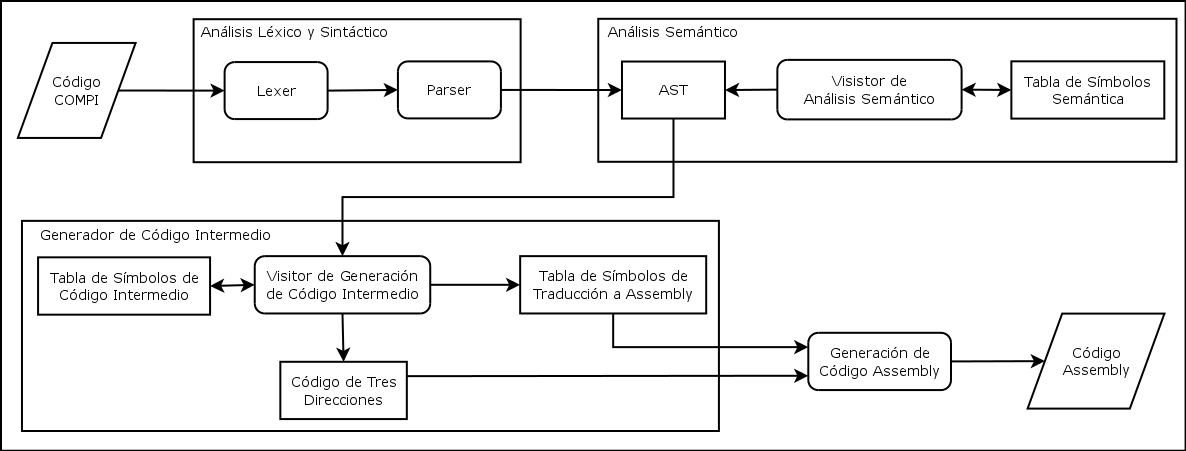
\includegraphics[width=\textwidth]{architecture.png}
    \caption{Arquitectura de COMPI}
    \label{fig:architecture}
  \end{figure}

  A partir del código fuente en COMPI, el primer paso se da a través del {\bf
  análisis léxico y sintáctico}. El lexer determina los tokens a procesar,
  identificando palabras reservadas, literales, etc. Esto se hace mediante la
  herramienta {\tt flex}. Se sigue del parser, que toma los elementos devueltos
  por el lexer y, siguiendo la gramática definida para el lenguaje, crea los
  nodos del árbol sintáctico. La herramienta que se encarga de parsear es {\tt
  bison}.

  Una vez terminada la etapa de análisis léxico y sintáctico, se sigue la etapa
  de {\bf análisis semántico}. La etapa arranca a partir del {\em abstract
  syntax tree} (AST o árbol sintáctico abstracto), que fue generado en la etapa
  anterior por el parser. Sobre el AST obtenido se aplica un {\em patrón
  visitor}, que crea y utiliza una tabla de símbolos localmente para comprobar
  distintos elementos de la semántica del lenguaje: tipos y alcance/visibilidad
  de los identificadores, asignaciones, número de parámetros y valor de retorno
  en las funciones, etc. Además de revisar con detenimiento ciertas reglas
  semánticas, como la declaración de identificadores y su llamada, la existencia
  de un método {\em main}, la correcta declaración de arreglos, entre otras
  restricciones definidas en las descripciones del lenguaje.

  Concluída la verificación semántica del AST pasamos a la etapa de {\bf
  generación de código intermedio}. El AST es recorrido nuevamente por un {\em
  patrón visitor}, que en este punto busca generar el código intermedio,
  definido como un código de tres direcciones. A través de una tabla de símbolos
  interna al proceso, se guarda información del alcance de los identificadores,
  así como cualquier otra información necesaria para luego generar el código
  intermedio de tres direcciones (e.g., tipo de la variable, el offset dentro
  del cuerpo del método, las variable, etc.). Este proceso genera dos recursos:
  el código de tres direcciones, que viene a ser el código intermedio de la
  aplicación y la tabla de traducción de símbolos para la traducción a Assembly,
  que guarda directamente información sobre las variables a utilizar en el
  código assembly.

  A partir de los recursos generados en la parte anterior se entra en la etapa
  de {\bf generación de código assembly}, que producirá un archivo en código
  assembly que luego será compilado mediante el compilador correspondiente.

  \section{Decisiones de Diseño}\label{sec:design}

  \subsection{Análisis sintáctico y AST}

  Para la creación del AST nos basamos en la estructura propuesta en la serie de
  posts de la página {\em gnuu}, llamado ``Writing Your Own Toy Compiler Using
  Flex, Bison and
  LLVM''\footnote{\url{http://gnuu.org/2009/09/18/writing-your-own-toy-compiler/}}.
  Este fue adaptado a los requerimientos del lenguaje COMPI. Todos los nodos
  heredan de una clase principal {\tt node} que a grandes razgos se diferencia
  entre declaraciones (de métodos y variables), órdenes de flujo ({\em
  statements}, en inglés) y expresiones (matemáticas, comparativas, lógicas).
  Hay algunas enumeraciones para definir los tipos (int, bool, float, etc.), los
  operadores relacionales (suma, resta, igual, distinto, y, o, etc.) y
  finalmente operadores de asignación. Se definieron {\em smart pointers} sobre
  todas las clases para hacer más sencillo el manejo de memoria.

  \subsection{Patrón visitor}

  Antes de describir las decisiones de diseño tomadas en las etapas de  análisis
  semántico y generación de código intermedio, es preciso aclarar cierto
  mecanismo elegido para implementar dichas etapas: el módulo {\tt visitor} (declarado
  en {\tt src/visitor.h}).

	La clase visitor solo implementa 2 métodos: el modo de ``aceptar'' (visitar)
	una expresión y el modo de aceptar una sentencia, en ambos casos en función
	del tipo de cada una. El resto de los métodos de la clase son métodos
	virtuales, cuya implementación será establecida por las clases que hereden de
	visitor.

	Nótese también que las distintas clases en {\tt node.h} que representan cada
	uno de los constructos de un programa heredan (directamente o indirectamente)
	de la clase {\tt node}, la cual tiene una clase virtual accept, que recibe un
	parámetro de tipo visitor. La idea es que cada constructo de un programa
	defina la manera de ``aceptarlo''; es decir, de visitarlo mediante una entidad
	externa, en este caso de tipo visitor. Todos estas clases básicamente
	implementan accept como una llamada al método visit del visitor pasado como
	parámetro, con ellos mismos ({\tt *this}) como parámetros.

	De este modo, cada clase que herede de visitor define la manera de recorrer un
	programa, y computar lo que sea necesario. Teniendo esto en cuenta, véanse las
	decisiones tomadas en cada una de las 3 etapas siguientes del proceso de
	compilación; a saber, análisis semántico, generación de código intermedio y
	generación de código assembly.

  \subsection{Análisis semántico}

	El análisis semántico, según se pidió que se realice en la sección 3.7 de la
	descripción del lenguaje COMPI, se implementa fundamentalmente en la clase
	{\tt semantic\_analysis}, declarada en {\tt src/semantic\_analysis.h}. Dicha
	clase hereda de visitor, e implementa el modo de recorrer un programa (una
	estrucutra de tipo {\tt program\_pointer}, definido como {\tt
	std::shared\_ptr$<$node\_program$>$} en {\tt node.h}) chequeando las
	características semánticas requeridas por el lenguaje. Para realización de su
	trabajo, {\tt semantic\_analysis} contiene un atributo de tipo {\tt
	symtables\_stack}.

	La clase {\tt symtables\_stack} modela el scope actual dentro de un programa
	COMPI, mediante la creación de una pila de objetos de tipo symtable, cada uno
	de los cuales contiene un {\tt std::map} que asocia un identificador a su
	información correspondiente, contenida en un objeto de tipo {\tt
	symtable\_element}.

	Consideraciones a tener en cuenta en esta etapa:

  \begin{itemize}
    \item Por el modo en que se procesan los métodos y clases dentro de un
    programa COMPI (i.e., avanzando sintácticamente en el código fuente), es
    preciso actualizar la información asociada a objetos {\tt symtable\_element}
    de tipo {\tt T\_FUNCTION} o {\tt T\_CLASS} cada vez que se define un
    parámetro o atributo nuevo, respectivamente, a medida que se avanza en el
    análisis del programa. Con este fin fueron creados {\tt
    symtable\_element::put\_func\_param} y {\tt
    symtable\_element::put\_class\_field}.
  	\item Como se ha tomado la decisión de no permitir tipos de datos recursivos
  	(i.e., clases que contienen atributos que son objetos de la propia clase que
  	se está definiendo), entonces es preciso, a la hora de chequear que la
  	definición de un atributo en una clase, saber el nombre de la clase que se
  	está definiendo. Esto se realiza mediante {\tt symtable::is\_recursive}.
  	\item No se pueden definir dos identificadores iguales dentro de una sola
  	symtable, y el método {\tt symtable::id\_exists} chequea esto.
  	\item El análisis del scope creado por las funciones se implementa mediante
  	{\tt symtables\_stack::put\_fun}, {\tt symtables\_stack::put\_func\_param} y
  	{\tt symtables\_stack::finish\_func\_analysis}. Análogamente, el análisis
  	del scope de las clases se realia mediante {\tt
  	symtables\_stack::put\_class}, {\tt symtables\_stack::put\_class\_field} y
  	{\tt symtables\_stack::finish\_class\_analysis}. De este modo, la resolución
  	de scopes es transparente para el usuario de {\tt symtables\_stack}.
  \end{itemize}

  \subsection{Generación de código intermedio}

	Ésta se realiza, fundamentalmente, en la clase {\tt inter\_code\_gen\_visitor}
	(la cual hereda de la clase visitor también) declarada en {\tt
	src/inter\_code\_gen\_visitor.h}. Esta clase implementa el modo de generar
	código intermedio para cierto constructo de un programa COMPI (constructo el
	cual se encuentra representado como objeto de alguna de las clases declaradas
	en {\tt src/node.h}).

	Se utilizan las constantes definidas en {\tt src/constants.h} (valores
	iniciales de las variables, y espacio ocupado por cada tipo de variable).

	Además, se ha implementado un módulo {\tt three\_address\_code} (en {\tt
	src/three\_address\_code.h}) donde se definen varios tipos de datos que se
	utilizarán en la generación de código intermedio. El principal es struct quad,
	que será la forma en que hemos optado representar a las instrucciones de
	código intermedio: consiste de un tipo de instrucción, un operador
	(correspondiente a ese tipo de instrucción) y 3 direcciones de memoria (varias
	instrucciones no usarán la totalidad de estas direcciones de memoria). Además,
	en este módulo se definen todas las funciones necesarias para construir o
	chequear propiedades de instrucciones de código intermedio ({\tt
	std::shared\_ptr$<$quad$>$}).

	Para generar código intermedio es necesario volver a modelar la resolución de
	scopes como se ha hecho en la etapa de análisis semántico, y este trabajo es
	realizado por una nueva clase: {\tt intermediate\_symtable} (declarada en {\tt
	src/intermediate\_symtable.h}).

	Pero {\tt intermediate\_symtable} no solo contiene un atributo de tipo {\tt
	symtables\_stack} para modelar la resolución de scopes, sino que también
	construye, a medida que se van generando las instrucciones de código
	intermedio (trabajo realizado por {\tt inter\_code\_gen\_visitor}), una tabla
	de símbolos (clase {\tt ids\_info}, también declarada en {\tt
	intermediate\_symtable.h}) que contiene información necesaria para
	posteriormente poder generar código assembly. Dicha información (almacenada en
	{\tt ids\_info}, con {\tt ids\_info::entry\_info} como principal reunión de
	datos) incluye: tipo de identificador (método, variable, variable temporal,
	etc.), tipo de dato, {\tt std::string} que representa el modo en que cierto
	identificador ha sido representado en la lista de instrucciones de código
	intermedio en cierto punto de scope, offset del identificador dentro del
	registro de activación al que pertenece (para posteriormente poder calcular la
	dirección exacta del identificador en memoria, en relación al valor de rbp en
	tiempo de ejecución), número de variables locales si se trata de un método
	(incluidas las variables temporales, que se almacenan en memoria también),
	clase a la que se pertenece si se trata de un método o un atributo, lista de
	atributos o de parámetros (si se trata de una clase o una función,
	respectivamente).

	Además, nótese que {\tt intermediate\_symtable} tiene una interfaz similar a
	la de {\tt symtables\_stack}, con el agregado de las funciones:

  \begin{itemize}
  	\item {\tt intermediate\_symtable::new\_label} (que devuelve una nueva
  	etiqueta auxiliar que el usuario podrá incorporar en su código intermedio
  	con la seguridad de ser	única),
  	\item {\tt intermediate\_symtable::set\_number\_vars} (que permite modificar
  	el número de variables, temporales o no, utilizadas en la función actual, lo
  	cual será útil posteriormente al generar el código assembly de registro de
  	activación para dicha función),
  	\item {\tt intermediate\_symtable::new\_temp} (que registra una nueva
  	variable temporal y le otorga una representación de tipo {\tt std::string}
  	única),
    \item {\tt intermediate\_symtable::get\_ids\_info} (que devolverá la tabla
    de símbolos con la información generada durante la generación de código
    intermedio, necesaria para la generación de código assembly).
  \end{itemize}

  \section{Generación de código assembly}

  Teniendo ya una lista de instrucciones de código intermedio junto a la tabla
  de símbolos (construida en la generación de dicha lista, y que contiene
  información necesaria para esta etapa), se procede a la generación de código
  intermedio mediante la clase {\tt asm\_code\_generator} (declarada en
  {\tt src/asm\_code\_generator.h}).

	Cabe aclarar aquí que se implementó el protocolo de stack frame (registro de
	activación) correspondiente al sistema {\tt V AMD64 ABI}. Dicho sistema
	establece que los primeros 6 parámetros que se desean pasar al llamar a una
	función son pasados los registros {\tt RDI}, {\tt RSI}, {\tt RDX}, {\tt RCX},
	{\tt R8} y {\tt R9}. Los restantes parámetros se pasan ``pusheándolos'' al
	stack frame. Técnicamente, el sistema {\tt V AMD64 ABI} otorga los 128 bytes
	siguientes a la dirección a la que apunta el registro {\tt RSP} para que los
	utilice la función en ejecución si le resulta necesario para almacenar
	variables temporales. Pero, por simplicidad, nuestro compilador guarda cada
	variable temporal en el stack frame, cargándolas en registros si es necesario
	computar algún valor sobre las variables temporales. Los resultados de tales
	cómputos también son guardados en el stack frame.

	Por último, observar que en el módulo {\tt asm\_instruction} ({\tt
	src/asm\_instruction.h}) se definen los tipos de datos análogos a los
	definidos en el módulo {\tt three\_address\_code}, pero para esta etapa.
	Contiene toda la información necesaria para poder generar la lista de
	instrucciones en assembly, junto a funciones (como {\tt
	print\_asm\_instructions\_list\_intel\_syntax}) que sirven para obtener,
	finalmente, el código assembly.

  \section{Conclusiones}\label{sec:conclusions}

  En términos generales tenemos un balance positivo de este trabajo. El proyecto
  fue de gran utilidad para entender el proceso de un compilador. Desde el
  diseño del lenguaje hasta la generación del código objeto. El resultado final
  fue el mismo compilador de COMPI que se encuentra disponible web.

  En el trabajo entregado buscamos seguir los lineamientos propuestos al
  principio de la materia en cuestión de diseño del lenguaje COMPI. Nos
  encontramos con algunos obstáculos, algunos de ellos los pudimos solucionar
  con facilidad y otros quedarían pendientes de disponer de mayor tiempo.

  La materia en sí mostró ser de gran utilidad, teniendo en cuenta el transfondo
  fuertemente teórico que esta carrera posee, trabajando nuevos conceptos, más
  en el campo de lo práctico que lo teórico.

\end{document}
